\documentclass[11pt, aspectratio=169]{beamer}
\usefonttheme[onlymath]{serif}

\setbeamersize{text margin left=1.5em}
\setbeamersize{text margin right=1.5em}

\setbeamertemplate{frametitle}{%
  \vskip1ex
  \usebeamerfont{frametitle}%
  \insertframetitle\par
  \vskip1ex
  \hrule
}

\setbeamertemplate{blocks}[rounded][shadow=true]

% Add numbered captions for figures/tables in beamer
\setbeamertemplate{caption}[numbered]

\setbeamertemplate{itemize item}{\usebeamerfont{itemize item}\textbullet}
\setbeamertemplate{itemize subitem}{\usebeamerfont{itemize subitem}\textbullet}
\setbeamertemplate{itemize subsubitem}{\usebeamerfont{itemize subsubitem}\textbullet}

\makeatletter
\geometry{%
  papersize={\fpeval{\beamer@paperwidth*1.5}pt,\fpeval{\beamer@paperheight*1.5}pt},
  hmargin=\fpeval{0.5 * 1.0}cm,% 1cm
  vmargin=0cm,%
  head=\fpeval{0.5*1.5}cm,% 0.5cm
  headsep=0pt,%
  foot=\fpeval{0.5*1.5}cm% 0.5cm
}
\makeatother

\usepackage{booktabs}
\usepackage{graphicx}
\usepackage[usenames,dvipsnames]{xcolor} % <-- add xcolor so \textcolor works
\usepackage{amsmath}
\usepackage{amssymb}
\usepackage{mathtools}

\usepackage[
  backend=bibtex,
  style=authoryear,   % or numeric
  citestyle=authoryear
]{biblatex}
\addbibresource{../../references.bib}

% Your custom commands (kept as is)
\newcommand{\mrm}[1]{\mathrm{#1}}
\newcommand{\mbb}[1]{\mathbb{#1}}
\newcommand{\mb}[1]{\mathbf{#1}}
\newcommand{\mc}[1]{\mathcal{#1}}
\newcommand{\tb}[1]{\textbf{#1}}
\newcommand{\Unif}{\operatorname{Unif}}

\title{An Improvement to Conservative Q-Learning}
\author{Gwanwoo Choi}
\institute{MLIC}
\date{} % To use the current date

\begin{document}

\begin{frame}
    \titlepage
\end{frame}


% https://tex.stackexchange.com/questions/541559/citep-vs-parencite
% \citep - \parencite
% \citet - \textcite
% \citealp - \citealt - \cite


\begin{frame}{Offline Learning}
  \begin{block}{Preliminaries of Offline Reinforcement Learning}
    \itemize{
        \item Markov Decision Process (MDP): $(\mc{S}, \mc{A}, p, r, \gamma)$
        \item State space: $\mc{S}$, Action space: $\mc{A}$
        \item Transition dynamics: $p(s^\prime|s,a)$, Reward function: $r(s,a)$
        \item Discount factor: $\gamma \in [0,1)$
        \item Policy: $\pi(a|s)$, Behavior Policy: $\beta(a|s)$
        \item In offline RL, we cannot interact with the environment during training. We have access to only a static dataset $\mc{D} = \{(s_i, a_i, r_i, s_i^\prime)\}_{i=1}^N$ collected by an unknown behavior policy $\beta$.
        \item Goal: Find the optimal policy $\pi^*$ that maximizes cumulative discounted reward at \tb{test time}.
        $$J(\pi) = \mbb{E}_{\substack{s_0 \sim p_0 \\ a_t \sim \pi(\cdot|s_t) \\ s_{t+1} \sim p(\cdot|s_t,a_t)}}\left[\sum_{t=0}^\infty \gamma^t r(s_t,a_t)\right]$$
    }
  \end{block}
  % }
\end{frame}

\begin{frame}{Offline Learning}
    \begin{block}{Problem of Offline RL}
    \itemize{
        \item Offline RL: Learn a policy from a static dataset $\mc{D}$ collected by an unknown behavior policy $\beta$.
        \item In offline learning, we cannot know the real transition dynamics $p(s^\prime|s,a)$. Thus, critic learning occurs only on in-distribution $(s,a)$ state-action pairs from the dataset $\mc{D}$.
        $$
          \min_\theta \mbb{E}_{\substack{(s,a,r,s^\prime) \sim \mc{D} \\ a^\prime \sim \pi_\phi} }\left[ (r + \gamma Q_\theta(s^\prime, a^\prime)  - Q_\theta (s,a))^2\right]
        $$

        \item One problem in offline RL is that unseen state-action pairs $(s,a) \sim \pi$ lead to errors due to untrustworthy function approximation. 
        
        \item In offline RL, not all state-action points may be included in the dataset $\mc{D}$, forcing the $Q$ function to extrapolate. This can cause large errors that accumulate through the Bellman update:
        $$
          \min_\theta \mbb{E}_{\substack{(s,a,r,s^\prime) \sim \mc{D} \\ \textcolor{red}{a^\prime \sim \pi_\phi}} }\left[ (r + \gamma \textcolor{red}{Q_\theta(s^\prime, a^\prime)}  - Q_\theta (s,a))^2\right]
        $$
    }
  \end{block}
\end{frame}

\begin{frame}{Out-of-Distribution Problem}
    \begin{block}{OOD problem}
      Suppose we learn the $Q$ function using Soft Actor-Critic (SAC), an online algorithm, in an \tb{offline setting}.
      \begin{itemize}
        \item The SAC objective consists of policy improvement and Q-function learning:
        $$
        \begin{gathered}
        \textcolor{violet}{\min_\phi} \mbb{E}_{\substack{s \sim \mc{D} \\ a \sim \pi_\phi}}\left[\alpha \log \pi_\phi(a|s) \textcolor{violet}{- Q_\theta(s,a)}\right] \\
        \min_\theta \mbb{E}_{\substack{(s,a,r,s^\prime) \sim \mc{D} \\ \textcolor{red}{a^\prime \sim \pi_\phi}} }\left[ (r + \gamma \textcolor{red}{Q_\theta(s^\prime, a^\prime)}  - Q_\theta (s,a))^2\right]
        \end{gathered}
        $$
        \item \tb{Key question}: Is $\textcolor{red}{Q_\theta (s^\prime, a^\prime)}$ reliable when $(s^\prime, a^\prime)$ is \textcolor{red}{out-of-distribution}?
        \item If $(s^\prime, a^\prime)$ is OOD, $Q_\theta(s^\prime, a^\prime)$ is often \tb{overestimated} due to extrapolation.
        \item This overestimation propagates: $Q(s,a) \leftarrow r + \gamma Q(s^\prime, a^\prime)$, compounding errors.
        \item The policy then exploits \textcolor{violet}{overestimated Q-values}, selecting poor actions that appear artificially good.


        % \item Is $\textcolor{red}{Q_\theta (s^\prime, a^\prime)}$ trustworthy? What if $(s^\prime, a^\prime)$ is \textcolor{red}{out-of-distribution}?
        % \item Suppose that, unfortunately, $Q(s^\prime, a^\prime)$ is \tb{highly approximated} for an OOD point $(s^\prime, a^\prime)$.
        % \item Then this overestimation error propagates through bootstrapping: $Q(s,a) \leftarrow r + \gamma Q(s^\prime, a^\prime)$.
        % \item Also, \textcolor{violet}{overestimated $Q$} values lead to suboptimal policy updates in the policy improvement step. \textcolor{gray}{(why?)}
        % % \item If $(s^\prime, a^\prime)$ is OOD, then $Q_\theta(s^\prime, a^\prime)$ tends to be \tb{overestimated} due to extrapolation errors in function approximation. The policy $\pi_\phi$ then exploits these overestimated values, leading to performance degradation.
      \end{itemize}
    \end{block}
\end{frame}

\begin{frame}{Conservative Q Learning}
  \begin{block}{Conservative Q Learning \parencite{kumarConservativeQLearningOffline2020} Motivation}
    
    \tb{Goal}: Prevent overestimation by making Q-values \tb{conservative} for OOD actions.
    % \tb{Key question}: Is $\textcolor{red}{Q_\theta (s^\prime, a^\prime)}$
    % How can we solve the OOD \& overestimation problem?
    \begin{itemize}
      \item \tb{Key insight}: Actions from policies different from $\beta$ are more likely to be OOD.
      \item Consider an arbitrary policy $\mu \neq \beta$. For $s \sim \mc{D}$ and $a \sim \mu(\cdot|s)$, the pair $(s,a)$ may be OOD.
      \item \tb{Approach(1)}: Lower Q-values for actions under $\mu$ while keeping them accurate for actions in $\mc{D}$:
      \item \tb{Objective(1)}: Penalize Q-values for actions sampled from $\mu$:
      \begin{equation}
        \min_\theta \max_\mu  \underbrace{\alpha^\prime \mbb{E}_{\substack{s \sim \mc{D} \\ a \sim \mu}}\left[Q_\theta(s,a)\right]}_{\text{Conservatism penalty}} + \underbrace{\frac{1}{2}\mbb{E}_{\substack{(s,a,r,s^\prime) \sim \mc{D} \\ a^\prime \sim \pi_\phi}}\left[\left(r + \gamma Q_\theta(s^\prime, a^\prime) - Q_\theta(s,a)\right)^2\right]}_{\text{Standard Bellman error}} + \underbrace{\mc{R}(\mu)}_{\text{Regularizer on } \mu}
      \end{equation}
        % \min_\theta \max_\mu \left\{ \alpha \mbb{E}_{s \sim \mc{D}, a \sim \mu}[Q_\theta(s,a)] - \mbb{E}_{(s,a) \sim \mc{D}}[Q_\theta(s,a)] \right\}
      \item This encourages conservative Q-estimates for OOD actions.
      \item However, this objective \tb{can hurt Q-values for in-distribution actions} $a \in \mc{D}$.
      \item \tb{Approach(2)}: Do not penalize Q-values for in-distribution actions.
      \item \tb{Objective(2)}: Depenalize Q-values for in-distribution actions:
      \begin{equation}
          \min_\theta \max_\mu  \underbrace{\alpha \left(\mbb{E}_{\substack{s \sim \mc{D} \\ a \sim \mu}}\left[Q_\theta(s,a)\right] - \mbb{E}_{(s,a) \sim \mc{D}}[Q_\theta(s,a)]\right)}_{\text{More loosen conservatism penalty}} + \underbrace{\frac{1}{2}\mbb{E}_{\substack{(s,a,r,s^\prime) \sim \mc{D} \\ a^\prime \sim \pi_\phi}}\left[\left(r + \gamma Q_\theta(s^\prime, a^\prime) - Q_\theta(s,a)\right)^2\right]}_{\text{Standard Bellman error}} + \underbrace{\mc{R}(\mu)}_{\text{Regularizer on } \mu}
      \end{equation}
    \end{itemize}
  \end{block}
\end{frame}

\begin{frame}{Conservative Q Learning}
  \begin{block}{Conservative Q Learning Framework}
    \begin{itemize}
      \item Especially, in this presentation, I focus on \tb{continuous action space}.
      \item \tb{Policy Evaluation}: Learn conservative Q-function by minimizing the CQL objective:
      $$
        \min_\theta \max_\mu  \alpha^\prime \left(\mbb{E}_{\substack{s \sim \mc{D} \\ a \sim \mu}}\left[Q_\theta(s,a)\right] - \mbb{E}_{(s,a) \sim \mc{D}}[Q_\theta(s,a)]\right) + \frac{1}{2}\mbb{E}_{\substack{(s,a,r,s^\prime) \sim \mc{D} \\ a^\prime \sim \pi_\phi}}\left[\left(r + \gamma Q_\theta(s^\prime, a^\prime) - Q_\theta(s,a)\right)^2\right] + \mc{R}(\mu)
      $$
      \item \tb{Policy Improvement}: Update policy via maximizing expected Q-values (SAC style):
      $$
        \min_\phi \mbb{E}_{\substack{s \sim \mc{D} \\ a \sim \pi_\phi}}\left[\alpha \log \pi_\phi(a|s) {- Q_\theta(s,a)}\right]
      $$
    \end{itemize}
  \end{block}
\end{frame}

\begin{frame}{Conservative Q Learning}
  \begin{block}{CQL($\mc{H}$)}
    \begin{itemize}
      \item Special case of CQL framework when choosing $\mc{R}(\mu) = \mc{H}(\mu)$. It can be shown that the optimal $\mu^\ast(a|s) = \exp(Q(s,a))$
      \item \tb{Policy Evaluation}: We can estimate $\log\sum_q \exp(Q(s,a))$ by \textcolor{red}{importance sampling}.
      \begin{equation*}
        \begin{gathered}
          \min_\theta  \alpha^\prime \mbb{E}_{s \sim \mc{D}}\left[\textcolor{red}{\log \sum_a \exp(Q_\theta(s,a))} - \mbb{E}_{a \sim \beta(a|s)}[Q_\theta(s,a)]\right] + \frac{1}{2}\mbb{E}_{\substack{(s,a,r,s^\prime) \sim \mc{D} \\ a^\prime \sim \pi_\phi}}\left[\left(r + \gamma  Q_\theta(s^\prime, a^\prime) - Q_\theta(s,a)\right)^2\right] \\ 
          \approx \min_\theta \alpha \mbb{E}_{(s,a) \sim \mc{D}}\left[\textcolor{red}{w_{\theta, \phi}(s)} - Q_\theta(s,a) \right] + \frac{1}{2}\mbb{E}_{\substack{(s,a,r,s^\prime) \sim \mc{D} \\ a^\prime \sim \pi_\phi}}\left[\left(r + \gamma Q_\theta(s^\prime, a^\prime) - Q_\theta(s,a)\right)^2\right] \\
          \text{where } \textcolor{red}{w_{\theta, \phi}(s)} = \log \left( \frac{1}{3N} \sum^N_{a_i \sim \Unif(a)}\left[\frac{\exp(Q_\theta(s,a_i))}{\Unif(a_i)}\right] + \frac{1}{3N} \sum_{a_i \sim \pi_\phi(a|s)}^N\left[\frac{\exp(Q_\theta(s, a_i))}{\pi_\phi(a_i|s)}\right] + \frac{1}{3N} \sum_{a^\prime_i \sim \pi_\phi(a^\prime|s^\prime)}^N \left[\frac{\exp(Q_\theta(s^\prime, a^\prime_i))}{\pi_\phi(a^\prime_i|s^\prime)}\right] \right)
        \end{gathered}
      \end{equation*}
        
      \item \tb{Policy Improvement}:
      $$
        \min_\phi \mbb{E}_{\substack{s \sim \mc{D} \\ a \sim \pi_\phi}}\left[\alpha \log \pi_\phi(a|s) {- Q_\theta(s,a)}\right]
      $$
    \end{itemize}
  \end{block}
\end{frame}

\begin{frame}{Conservative Q Learning}
  \begin{block}{Recall: $w(s)$ equation}  
    \begin{equation*}
      w_{\theta, \phi}(s) = \log \left( \frac{1}{3N} \sum^N_{a_i \sim \Unif(a)}\left[\frac{\exp(Q_\theta(s,a_i))}{\Unif(a_i)}\right] + \frac{1}{3N} \sum_{a_i \sim \pi_\phi(a|s)}^N\left[\frac{\exp(Q_\theta(s, a_i))}{\pi_\phi(a_i|s)}\right] + \frac{1}{3N} \sum_{a^\prime_i \sim \pi_\phi(a^\prime|s^\prime)}^N \left[\frac{\exp(Q_\theta(s^\prime, a^\prime_i))}{\pi_\phi(a^\prime_i|s^\prime)}\right] \right)
    \end{equation*}
  \end{block}
  \begin{block}{CQL($\mc{H}$) Lagrangian}
    \begin{itemize}
      \item Fixed alpha is sometimes not gooe for complicated tasks.
      \item Inestead of using fixed $\alpha^\prime$, make \textcolor{red}{$\alpha^\prime$} also \textcolor{red}{learnable parameter}. (Lagrangian dual problem)
      \item \tb{Policy Evaluation}: In Lagrangian dual form, $\alpha^\prime$ is trainable parameter and \textcolor{red}{$\tau$ is fixed constant}. If training becomes success, $w(s,a) - \mbb{E}_{a \sim \beta(a|s)}[Q(s,a)]$ converges to $\tau$.
      \begin{equation*}
        \begin{gathered}
          \min_\theta \textcolor{red}{\alpha^\prime} \left(\mbb{E}_{(s,a) \sim \mc{D}} \left[w_{\theta, \phi}(s) - Q_\theta(s,a)\right] - \textcolor{red}{\tau}\right) + \frac{1}{2}\mbb{E}_{\substack{(s,a,r,s^\prime) \sim \mc{D} \\ a^\prime \sim \pi_\phi}}\left[\left(r + \gamma  Q_\theta(s^\prime, a^\prime) - Q_\theta(s,a)\right)^2\right] \\
          \implies \begin{cases}
          \min_\theta \alpha^\prime (\mbb{E}_{(s,a) \sim \mc{D}}[w_{\theta, \phi}(s) - Q_\theta(s,a)] - \tau) + \frac{1}{2}\mbb{E}_{\substack{(s,a,r,s^\prime) \sim \mc{D} \\ a^\prime \sim \pi_\phi}}\left[\left(r + \gamma Q_\theta(s^\prime, a^\prime) - Q_\theta(s,a)\right)^2\right] \\
          \min_{\textcolor{red}{\alpha^\prime}} \textcolor{red}{\alpha^\prime} (\mbb{E}_{(s,a) \sim \mc{D}}[w_{\theta, \phi}(s) - Q_\theta(s,a)] - \tau)
          \end{cases}
        \end{gathered}
      \end{equation*}
      \item \tb{Policy Improvement}:
      $$
        \min_\phi \mbb{E}_{\substack{s \sim \mc{D} \\ a \sim \pi_\phi}}\left[\alpha   \log \pi_\phi(a|s) {- Q_\theta(s,a)}\right]
      $$
    \end{itemize}
  \end{block}
\end{frame}


\begin{frame}{Idea}
  \begin{block}{CQL penalization term}
    \begin{itemize}
      \item In CQL($\mc{H}$), critic update rule is driven from following equation:
      \begin{equation*}
        \begin{gathered}
          \arg\min_\theta \alpha \left(\mbb{E}_{\substack{s \sim \mc{D} \\ a \sim \mu}}\left[Q_\theta(s,a)\right] - \mbb{E}_{(s,a) \sim \mc{D}}[Q_\theta(s,a)]\right) + \frac{1}{2}\mbb{E}_{\substack{(s,a,r,s^\prime) \sim \mc{D} \\ a^\prime \sim \pi_\phi}}\left[\left(r + \gamma Q_\theta(s^\prime, a^\prime) - Q_\theta(s,a)\right)^2\right] + \mc{R}(\mu) \\
          \begin{aligned}
            \forall (s,a) \sim \mc{D}, &\frac{\partial}{\partial Q_\theta(s,a)} \left[\alpha^\prime\left(\mbb{E}_{\substack{s \sim \mc{D} \\ a \sim \mu}}[Q_\theta(s,a)] - \mbb{E}_{\substack{s \sim \mc{D} \\ a \sim \beta}} \left[Q_\theta(s,a)\right]\right) + \frac{1}{2}\mbb{E}_{\substack{(s,a, r, s^\prime) \sim \mc{D} \\ a^\prime \sim \pi_\phi}} \left[(r + \gamma Q_\theta(s^\prime, a^\prime) - Q_\theta(s,a))^2\right]\right] = 0 \\
            &\implies \alpha^\prime \left(d^\beta(s) \left(\mu(a|s) - \beta(a|s)\right)\right) + d^\beta(s) \beta(a|s)\left(Q_\theta(s,a) - \mbb{E}_{\substack{s^\prime \sim \mc{D} \\ a^\prime \sim \pi_\phi}}[r + \gamma Q_\theta(s^\prime, a^\prime)]\right) =0 \\
            &\implies Q_\theta(s,a) \leftarrow \mbb{E}_{\substack{s^\prime \sim \mc{D} \\ a^\prime \sim \pi_\phi}}[r + \gamma Q_\theta(s^\prime, a^\prime)] - \textcolor{red}{\alpha^\prime \left\lvert \frac{\mu(a|s)}{\beta(a|s)} - 1 \right\rvert}
          \end{aligned}
        \end{gathered}
      \end{equation*}
      \item \textcolor{red}{$\alpha^\prime \left\lvert \frac{\mu(a|s)}{\beta(a|s)} - 1 \right\rvert$} is the key penalization term of CQL.
    \end{itemize}
  \end{block}
\end{frame}

\begin{frame}{Idea}
    \begin{block}{Change penalization term}
      \begin{itemize}
        \item The essence of CQL penalization is the term $\alpha^\prime \left\lvert \frac{\mu(a|s)}{\beta(a|s)} - 1 \right\rvert$:
        $$
           \forall (s,a) \sim \mc{D}, Q_\theta(s,a) \leftarrow \mbb{E}_{\substack{s^\prime \sim \mc{D} \\ a^\prime \sim \pi_\phi}}[r + \gamma Q_\theta(s^\prime, a^\prime)] - \alpha^\prime \left\lvert \frac{\mu(a|s)}{\beta(a|s)} - 1 \right\rvert
        $$
        \item Alternatively, I considered following penality term, which is based on $L_2$ distance between actions:
        \begin{equation*}
            \begin{aligned}  \forall (s,a) \sim \mc{D}, &Q_\theta(s,a) \leftarrow \mbb{E}_{\substack{s^\prime \sim \mc{D} \\ a^\prime \sim \pi_\phi}} \left[ r + \gamma Q_\theta (s^\prime, a^\prime) \right] - \textcolor{red}{\alpha^\prime \mbb{E}_{\hat{a}\sim \pi_\phi}[\left\lvert \hat{a} - a\right\rvert_2]} \\
              &\approx Q_\theta(s,a) \leftarrow \mbb{E}_{\substack{s^\prime \sim \mc{D} \\ a^\prime \sim \pi_\phi}} \left[ r + \gamma Q_\theta (s^\prime, a^\prime) \right]- \textcolor{red}{\frac{\alpha^\prime}{N} \sum^N_{\hat{a}_i \sim \pi_\phi}\left\lvert \hat{a}_i - a \right\rvert_2}
          \end{aligned}
        \end{equation*}
        Where $N$ is the number of sampled actions from policy $\pi$.
    \end{itemize}
  \end{block}
\end{frame}

\begin{frame}{Idea}
  \begin{block}{Recall: penalization terms}
    \begin{equation*}
      \begin{gathered}
        \forall (s,a) \sim \mc{D}, Q_\theta(s,a) \leftarrow \mbb{E}_{\substack{s^\prime \sim \mc{D} \\ a^\prime \sim \pi_\phi}}[r + \gamma Q_\theta(s^\prime, a^\prime)] - \alpha^\prime \left\lvert \frac{\mu(a|s)}{\beta(a|s)} - 1 \right\rvert \\
        \forall (s,a) \sim \mc{D}, Q_\theta(s,a) \leftarrow \mbb{E}_{\substack{s^\prime \sim \mc{D} \\ a^\prime \sim \pi_\phi}} \left[ r + \gamma Q_\theta (s^\prime, a^\prime) \right]- {\frac{\alpha^\prime}{N} \sum^N_{\hat{a}_i \sim \pi_\phi}\left\lvert \hat{a}_i - a \right\rvert_2}
      \end{gathered}
    \end{equation*}
  \end{block}
  \begin{block}{Motivation}
    \begin{itemize}
        \item I motivated from the fact that $\left \lvert \frac{\mu(a|s)}{\beta(a|s)} -1 \right \rvert$ only calculates the density ratio between two policies, but does not directly reflect the distance between actions.
        \item \underline{For example}, let assume $a_1, a_2 \in \mc{A}$ and $ \vert a_1 - a_2\vert_2 \approx 0$ and $\substack{\mu(a_1|s) = 0.9 \\ \beta(a_1|s) =0.1}, \substack{\mu(a_2|s)=0.1 \\  \beta(a_2|s)=0.9}$.
        \item In continuous action space, semantically $a_1$ and $a_2$ are almost same actions. But CQL penalization term gives \tb{huge} penalty for both actions since:
        \begin{equation*}
          \textcolor{red}{\left\lvert \frac{\mu(a_1|s)}{\beta(a_1|s)} - 1 \right\rvert = 8},  \left\lvert \frac{\mu(a_2|s)}{\beta(a_2|s)} - 1 \right\rvert = 0.2
        \end{equation*}
        \item In my method, $\textcolor{red}{\vert a_1 - a_2\vert \approx 0}$, which is quite smalle and matches the semantic of continuous action space.
    \end{itemize}
  \end{block}
\end{frame}

\begin{frame}{Method}  
  \begin{block}{Recall: CQL Framework}
    \begin{itemize}
      \item \tb{Policy Evaluation}:
      $$
        \min_\theta \max_\mu  \alpha^\prime \left(\mbb{E}_{\substack{s \sim \mc{D} \\ \textcolor{red}{a \sim \mu}}}\left[Q_\theta(s,a)\right] - \mbb{E}_{(s,a) \sim \mc{D}}[Q_\theta(s,a)]\right) + \frac{1}{2}\mbb{E}_{\substack{(s,a,r,s^\prime) \sim \mc{D} \\ a^\prime \sim \pi_\phi}}\left[\left(r + \gamma Q_\theta(s^\prime, a^\prime) - Q_\theta(s,a)\right)^2\right] + \mc{R}(\mu)
      $$
      \item \tb{Policy Improvement}:
      $$
        \min_\phi \mbb{E}_{\substack{s \sim \mc{D} \\ a \sim \pi_\phi}}\left[\textcolor{red}{\alpha \log \pi_\phi(a|s)} {- Q_\theta(s,a)}\right]
      $$
    \end{itemize}
  \end{block}
  \begin{block}{Framework 1: Ours (w/o KL reg.)}
    \begin{itemize}
      \item \tb{Policy Evaluation}:
      \begin{equation*}
        \min_\theta \mbb{E}_{(s,a,r,s^\prime) \sim \mc{D}} \left[ \left(Q_\theta(s,a) - \left(r + \gamma Q_\theta(s^\prime, a^\prime) - \frac{\alpha^\prime}{N} \sum_{\hat{a}_i \sim \pi_\phi}^N \left\lvert \hat{a}_i - a \right\rvert_2 \right)\right)^2\right]
      \end{equation*}
      \item \tb{Policy Improvement}: I \textcolor{red}{dropped the entropy term $\alpha \mbb{E}_{s \sim \mc{D}}[\mc{H}(\pi)]$} in policy learning.
      \begin{equation*}
        \min_\phi \mbb{E}_{\substack{s \sim \mc{D} \\ a \sim \pi_\phi}}\left[- Q_\theta(s,a)\right]
      \end{equation*}
      \item In my method, compared with CQL, since exploration distribution $\mu$ is removed, I \textcolor{red}{dropped the exploration term $\alpha \mbb{E}_{s \sim \mc{D}}[\mc{H}(\pi)]$} in policy improvement.
    \end{itemize}
  \end{block}
\end{frame}

\begin{frame}{Experiment}
  \begin{block}{Baseline}
    \begin{itemize}
      \item By lack of preparation time, I only implemented \underline{CQL($\mc{H}$)} and \underline{CQL($\mc{H}$)} Lagrangian as baselines.
      \item Since \tb{lot of code implementations of CQL are different}, I implemented CQL baselines \tb{from scratch} based on the original paper and original codebase.
    \end{itemize}
  \end{block}
  \begin{block}{Environment}
    \begin{itemize}
      \item Due to limited time, I only experimented on D4RL \parencite{fuD4RLDatasetsDeep2021} \tb{AntMaze-v2}.
      \begin{figure}
        \centering
        \includegraphics[width=0.4\textwidth]{antmaze.png}
        \caption{AntMaze Environment \parencite{fuD4RLDatasetsDeep2021}}
      \end{figure}
    \end{itemize}
  \end{block}
\end{frame}

\begin{frame}{Experiment}
  \begin{block}{Common Hyperparameter choices}
    \begin{itemize}    
      \item Optimizer: Adam
      \item Discount factor $\gamma$: $0.99$
      \item Target network update rate $\tau$: $0.005$
      \item Batch size: $256$
      \item Number of training steps: $1,000,000$
      \item Policy network: 3 hidden layers (same with \parencite{kumarConservativeQLearningOffline2020} official codebase), 256 units per layer, ReLU activation, Tanh Gaussian policy
      \item Q network: 3 hidden layers, 256 units per layer, ReLU activation
      \item Policy learning rate: $3e-5$
      \item Number of Q Ensemble: 2
      \item Number of seeds: 4
      \item Number of evaluation environments per seed: 8
    \end{itemize}
  \end{block}
\end{frame}

\begin{frame}{Experiment}
    \begin{table}
      \centering
      \resizebox{0.50\textwidth}{!}{
        \begin{tabular}{lccc}
        \toprule
          \textbf{Method} & CQL($\mc{H}$) & CQL($\mc{H}$) Lagrangian & Ours (w/o KL reg.) \\
          \midrule
          \textbf{AntMaze-umaze-v2} & 100  & 10 & 24.2     \\
          \textbf{AntMaze-umaze-diverse-v2}  & 86.1 & 46.3 & 0          \\
          \textbf{Antmaze-medium-play-v2} & 0 & 0 & 0 \\
          \textbf{Antmaze-medium-diverse-v2} & 0 & 0 & 0       \\
          \textbf{Antmaze-large-play-v2} & 0 & 0  & 0\\
          \textbf{Antmaze-large-diverse-v2} & 0  & 0  & 0 \\
          \bottomrule
        \end{tabular}
      }
      \caption{Performance comparison across different environments. \hyperref[frame:table1_hyperparameter]{(Appendix: Hyperparameter Settings)}}
    \label{tab:antmaze_results}
  \end{table}
\end{frame}

\begin{frame}{Experiment}
  \begin{block}{Recall: Ours (w/o KL reg.)}
    \begin{itemize}
      \item \tb{Policy Evaluation}:
      \begin{equation*}
        \min_\theta \mbb{E}_{(s,a,r,s^\prime) \sim \mc{D}} \left[ \left(Q_\theta(s,a) - \left(r + \gamma Q_\theta(s^\prime, a^\prime) - \frac{\alpha^\prime}{\textcolor{red}{N}} \sum_{\hat{a}_i \sim \pi_\phi}^N \left\lvert \hat{a}_i - a \right\rvert_2 \right)\right)^2\right]
      \end{equation*}
      \item \tb{Policy Improvement}:
      \begin{equation*}
        \min_\phi \mbb{E}_{\substack{s \sim \mc{D} \\ a \sim \pi_\phi}}\left[- Q_\theta(s,a)\right]
      \end{equation*}
    \end{itemize}
  \end{block}

  \bigskip
  \begin{columns}
    \begin{column}{0.4\textwidth}
      \begin{table}
        \centering
        \resizebox{0.95\textwidth}{!}{
          \begin{tabular}{lccc}
            \toprule
            \textbf{Dataset / \textcolor{red}{$N$}} & 5 & 10 & 25 \\
            \midrule
            \textbf{AntMaze-umaze-v2 } & 9.4 & 24.2 & 0 \\ 
            \textbf{AntMaze-umaze-diverse-v2 } & 0 & 0 & 0 \\
            \textbf{AntMaze-medium-play-v2 } & 0 & 0 & 0 \\
            \textbf{AntMaze-medium--v2 } & 0 & 0 & 0  \\
            \tb{Antmaze-large-play-v2} & 0 & 0 & 0  \\
            \tb{Antmaze-large-diverse-v2} & 0 & 0 & 0 \\
            \bottomrule
          \end{tabular}
        }
        \caption{Effect of varying number of sampled actions $N$.}
        \label{tab:N_effect}
      \end{table}
    \end{column}

    \begin{column}{0.6\textwidth}
      \begin{block}{Effect of $N$}
        \begin{itemize}
          \item It seems that there is no meaningful difference on varying $N$.
          \item I choose $N=10$ for other experiments.
        \end{itemize}
      \end{block}
    \end{column}
  \end{columns}
\end{frame}

\begin{frame}{Experiment}
  \begin{block}{Recall: Ours (w/o KL reg.)}
    \begin{itemize}
      \item \tb{Policy Evaluation}:
      \begin{equation*}
        \min_\theta \mbb{E}_{(s,a,r,s^\prime) \sim \mc{D}} \left[ \left(Q_\theta(s,a) - \left(r + \gamma Q_\theta(s^\prime, a^\prime) - \frac{\textcolor{red}{\alpha^\prime}}{N} \sum_{\hat{a}_i \sim \pi_\phi}^N \left\lvert \hat{a}_i - a \right\rvert_2 \right)\right)^2\right]
      \end{equation*}
      \item \tb{Policy Improvement}:
      \begin{equation*}
        \min_\phi \mbb{E}_{\substack{s \sim \mc{D} \\ a \sim \pi_\phi}}\left[- Q_\theta(s,a)\right]
      \end{equation*}
    \end{itemize}
  \end{block}

  \begin{table}
    \centering
    \resizebox{0.50\textwidth}{!}{
      \begin{tabular}{lcccc} % match number of columns (1 label + 4 settings)
      \toprule
      \textbf{Dataset (Q learning rate) / \textcolor{red}{$\alpha^\prime$}} & $10^{-12}$ & $0.003$ & $0.01$ & $0.03$ \\
      \midrule
      \textbf{AntMaze-umaze-v2 ($0.0001$)} & 0 & 0 & 0 & \tb{3.25} \\ % fill values or '-' placeholders
      \textbf{AntMaze-umaze-v2 ($0.0003$)} & 0 & \tb{14.6} & 9.375 & 0 \\
      \textbf{AntMaze-medium-play-v2 ($0.0001$)} & 0 & \tb{12.5} & 0 & 0 \\
      \textbf{AntMaze-medium-play-v2 ($0.0003$)} & \tb{3.1} & 0 & 0 & 0 \\
      \bottomrule
    \end{tabular}
  }
  \caption{Effect of varying $\alpha^\prime$.}
  \label{tab:alpha_effect}
  \end{table}
  \begin{block}{Effect of $\alpha^\prime$}
    \begin{itemize}
      \item It seems that L2 distance based penalization works (except for AntMaze-medium-play-v2).
    \end{itemize}
  \end{block}
\end{frame}

\begin{frame}{Experiment}
  \begin{block}{Recall: Ours (w/o KL reg.)}
    \begin{itemize}
      \item \tb{Policy Evaluation}:
      \begin{equation*}
        \min_\theta \mbb{E}_{(s,a,r,s^\prime) \sim \mc{D}} \left[ \left(Q_\theta(s,a) - \left(r + \gamma Q_\theta(s^\prime, a^\prime) - \frac{\alpha^\prime}{\textcolor{red}{N}} \textcolor{red}{\sum_{\hat{a}_i \sim \pi_\phi}^N \left\lvert \hat{a}_i - a \right\rvert_2 }\right)\right)^2\right]
      \end{equation*}
      \item \tb{Policy Improvement}:
      \begin{equation*}
        \min_\phi \mbb{E}_{\substack{s \sim \mc{D} \\ a \sim \pi_\phi}}\left[- Q_\theta(s,a)\right]
      \end{equation*}
    \end{itemize}
  \end{block}

  \begin{columns}
    \begin{column}{0.55\textwidth}
      \begin{figure}
        \centering
        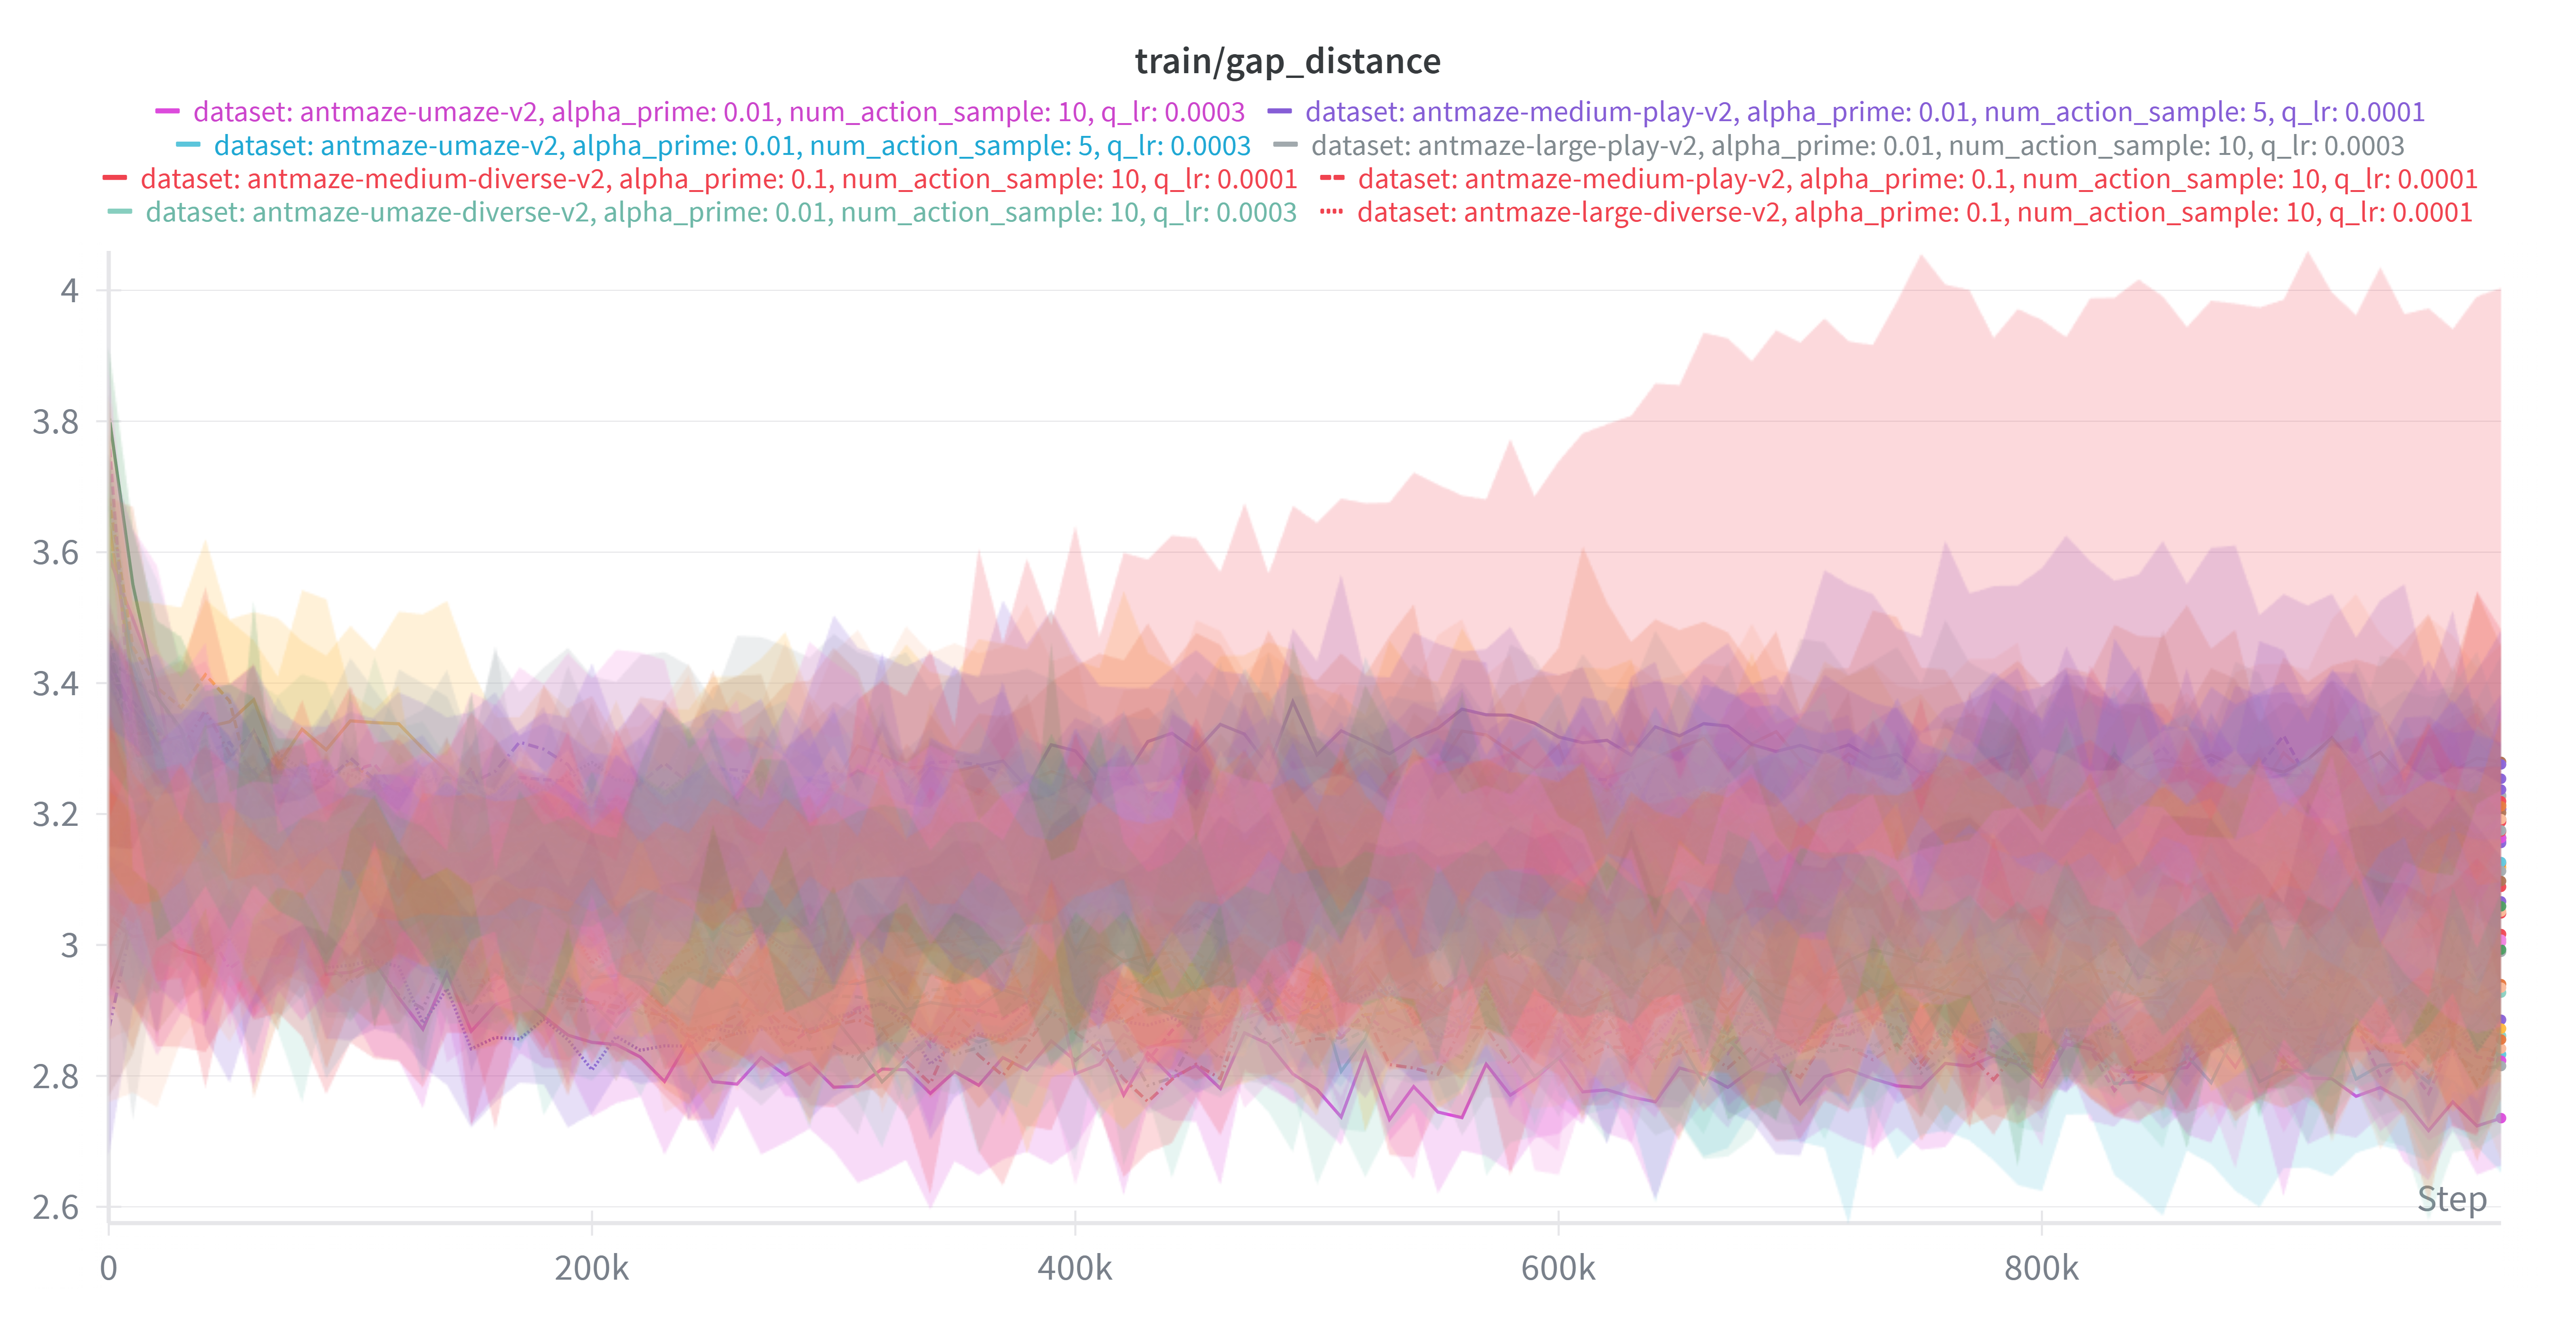
\includegraphics[width=1\textwidth]{gap_distance1.png}
        \caption{Learning curve of penalization term}
        \label{fig:gap_distance}
      \end{figure}
    \end{column}
    \begin{column}{0.35\textwidth}
      \begin{block}{Analysis}
        \begin{itemize}
          \item At first, I expect that penalization term converges to smaller value as training proceeds.
          \item However, as shown in the figure, penalization term \tb{keep} scales as training proceeds.
          \item It seems that an \tb{additional regularization term for the policy} needs to be applied.
        \end{itemize}
      \end{block}
    \end{column}
  \end{columns}
\end{frame}

\begin{frame}{Method}
  \begin{block}{Framework 2: Ours (w/ KL reg.)}
    \begin{itemize}
      \item \tb{Policy Evaluation}:
      \begin{equation*}
        \min_\theta \mbb{E}_{(s,a,r,s^\prime) \sim \mc{D}} \left[ \left(Q_\theta(s,a) - \left(r + \gamma Q_\theta(s^\prime, a^\prime) - \frac{\alpha^\prime}{N} \sum_{\hat{a}_i \sim \pi_\phi}^N \left\lvert \hat{a}_i - a \right\rvert_2 \right)\right)^2\right]
      \end{equation*}
      \item \tb{Policy Improvement}: I add \tb{KL regularization term} in policy learning.
      \begin{equation*}
        \min_\phi \mbb{E}_{\substack{s \sim \mc{D} \\ a \sim \pi_\phi}}\left[- Q_\theta(s,a) + \textcolor{red}{\alpha D_{KL}(\pi_\phi(\cdot|s) || \beta(\cdot|s))}\right]
      \end{equation*}
      This objective is \tb{infeasible} because behavior policy \tb{$\beta$ is unknown}.
      So I approximate it with \tb{lagrangian dual} form of KL divergence:
      \begin{equation*}
        \implies 
        \begin{cases}
          \min_\phi \mbb{E}_{\substack{(s,a) \sim \mc{D} \\ \hat{a} \sim \pi_\phi}}\left[-Q_\theta (s,a) - \alpha \left((\log \pi_\phi(\hat{a}|s) - \log \pi_\phi(a|s)) - \tau \right)\right] \\
          \min_\alpha \mbb{E}_{\substack{(s, a) \sim \mc{D} \\ \hat{a} \sim \pi_\phi}} \left[ - \alpha ((\log \pi_\phi(\hat{a}|s) - \log \pi_\phi(a|s)) - \tau) \right]
        \end{cases}
      \end{equation*}
      $\tau$ is a fixed threshold hyperparameter.
    \end{itemize}
  \end{block}
\end{frame}

\begin{frame}{Experiment}
    \begin{table}
      \centering
      \resizebox{0.65\textwidth}{!}{
        \begin{tabular}{lcccc}
        \toprule
          \textbf{Method} & CQL($\mc{H}$) & CQL($\mc{H}$) Lagrangian & Ours (w/o KL reg.) & CQL($\mc{H}$) (w/ KL reg.)\\
          \midrule
          \textbf{AntMaze-umaze-v2} & 100 & 10 & 24.2 &  78  \\
          \textbf{AntMaze-umaze-diverse-v2}  & 86.1 & 46.3 & 0 & 0        \\
          \textbf{Antmaze-medium-play-v2} & 0 & 0 & 0 & 20.1 \\ 
          \textbf{Antmaze-medium-diverse-v2} & 0 & 0 & 0 &  34.4    \\
          \textbf{Antmaze-large-play-v2} & 0 & 0  & 0 & 0 \\
          \textbf{Antmaze-large-diverse-v2} & 0  & 0  & 0 & 0 \\
          \bottomrule
        \end{tabular}
      }
      \caption{Performance comparison across different environments (Hyperparameter settings in Appendix \hyperref[frame:table1_hyperparameter]{Appendix: Hyperparameter Settings}).}
    \label{tab:antmaze_results2}
  \end{table}

  \begin{figure}
    \centering
    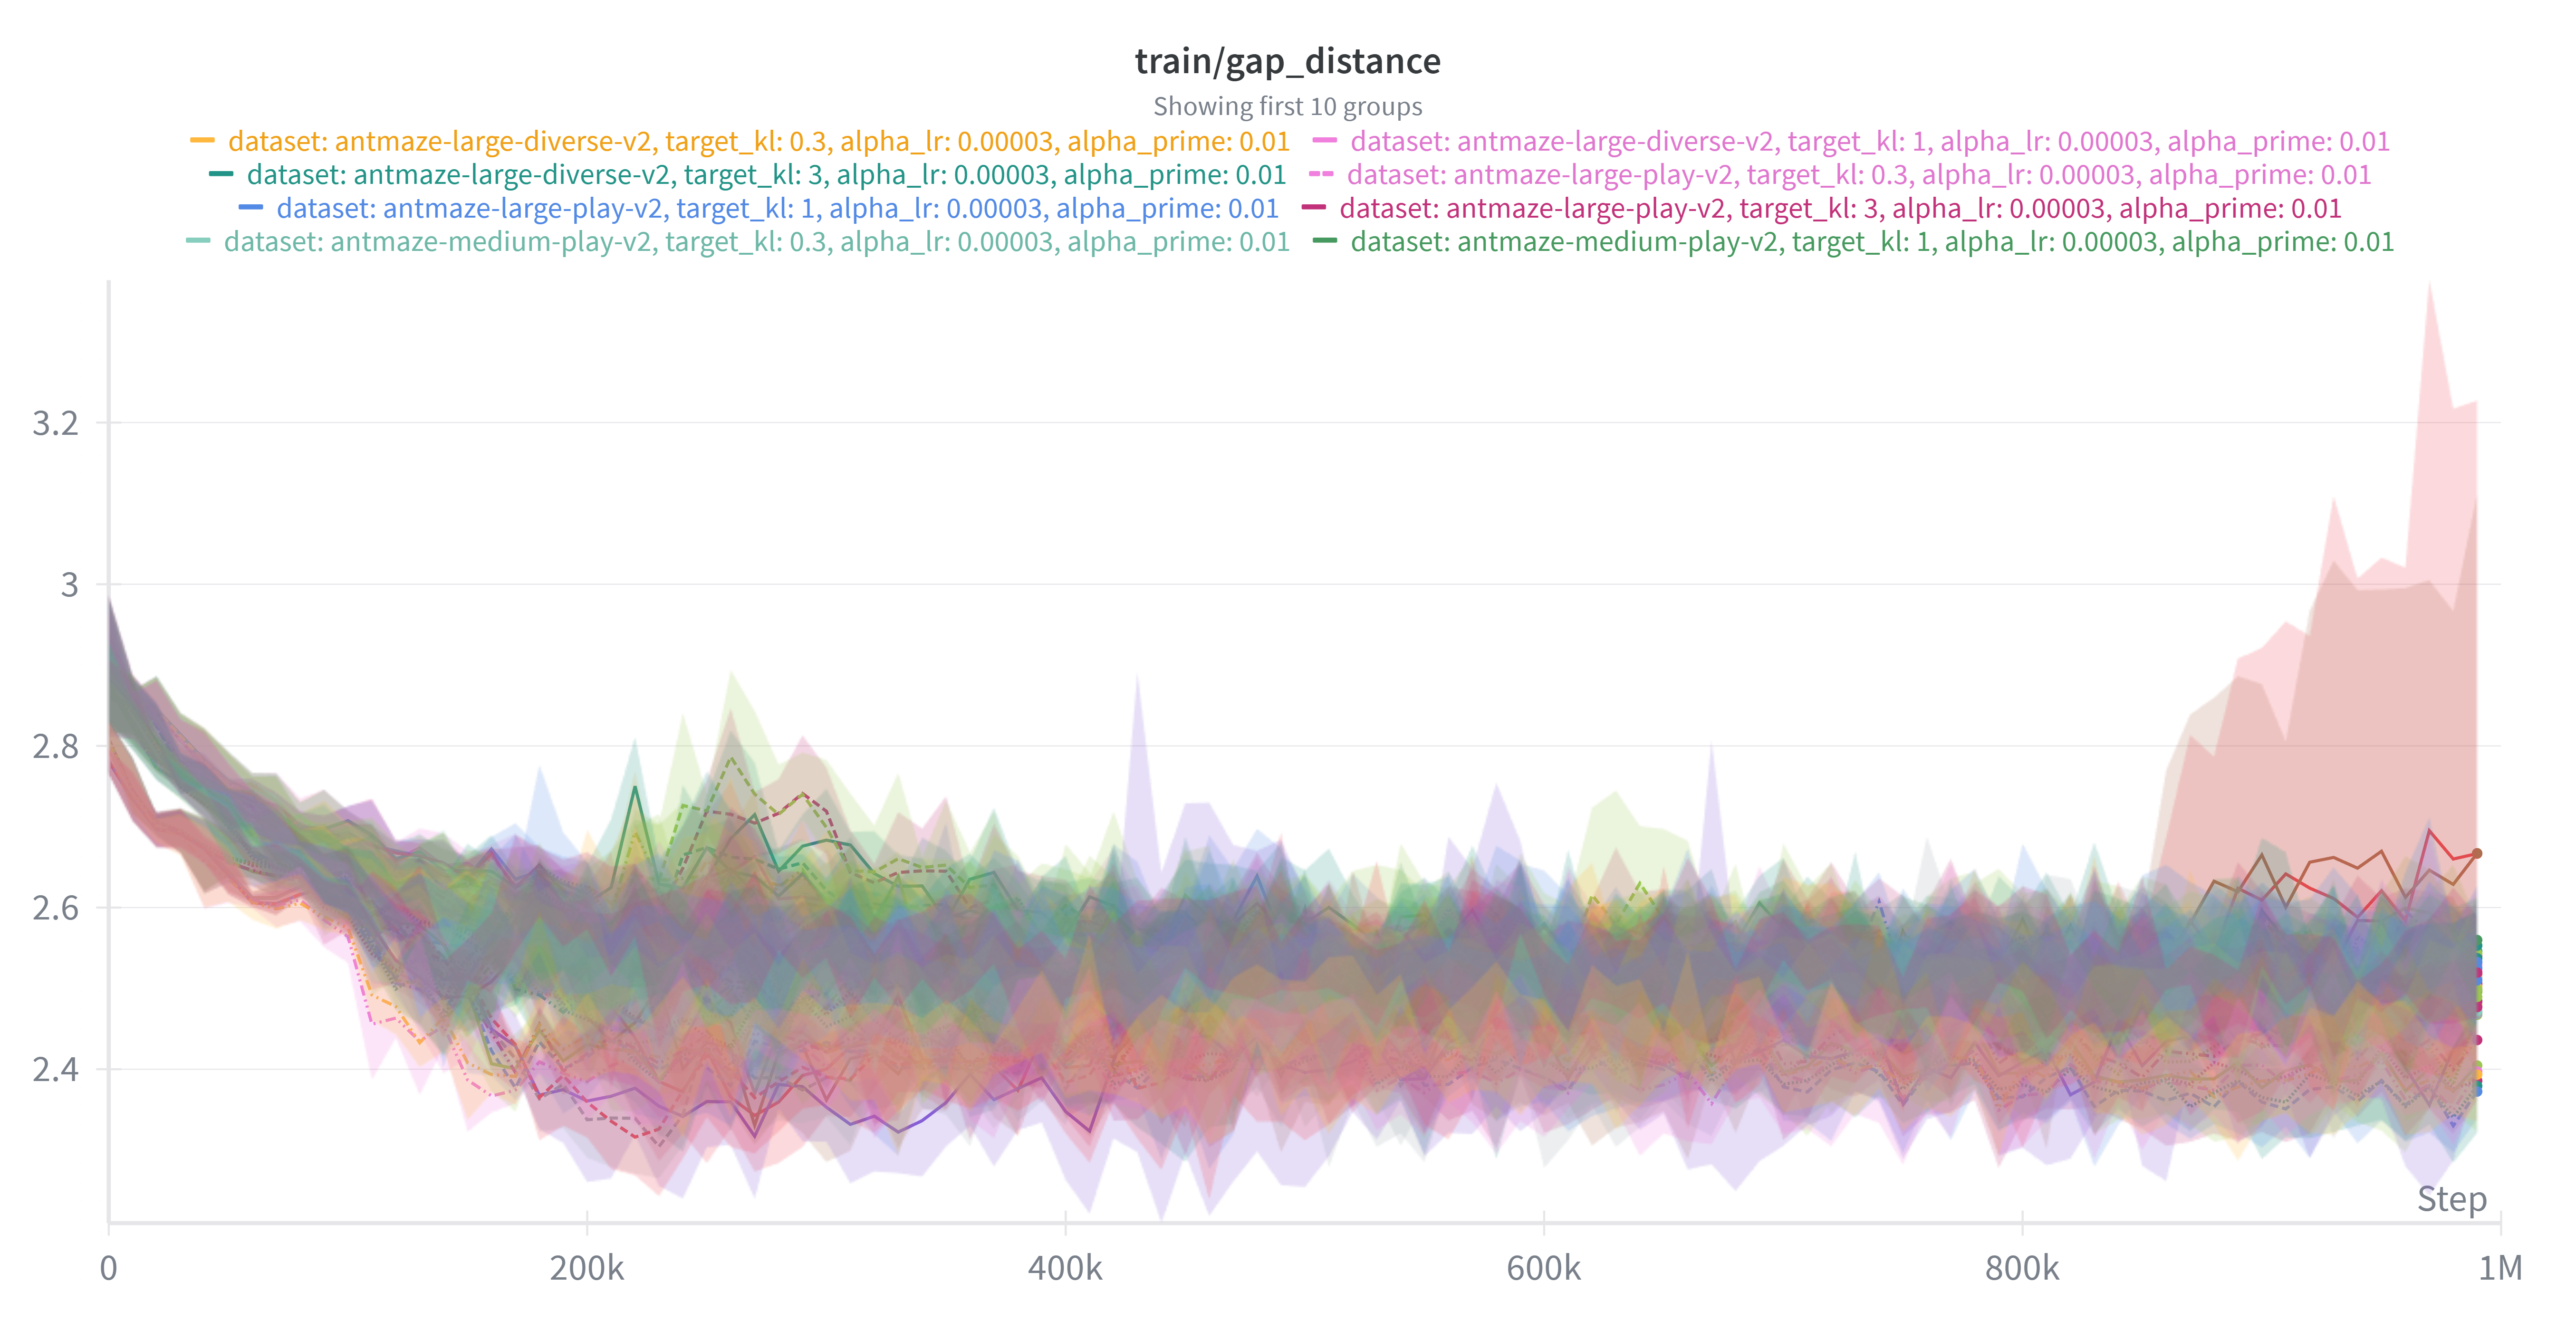
\includegraphics[width=0.5\textwidth]{gap_distance2.png}
    \caption{Learning curve of penalization term with KL regularization}
    \label{fig:gap_distance2}
  \end{figure}
\end{frame}



% \begin{frame}{Table example}
%   \begin{table}
%     \centering
%     \resizebox{0.9\textwidth}{!}{
%       \begin{tabular}{lcccc}
%       \toprule  % 맨 위 굵은 선
%                 \textbf{Method} & \textbf{Env 1} & \textbf{Env 2} & \textbf{Env 3} & \textbf{Avg. Score} \\
%                 \midrule  % 중간 얇은 선
%                 DQN             & 120.5          & 85.2           & -10.4          & 65.1 \\
%                 PPO             & 250.1          & 110.5          & 55.2           & 138.6 \\
%                 \textbf{Ours}   & \textbf{310.8} & \textbf{145.3} & \textbf{98.7}  & \textbf{184.9} \\
%                 \bottomrule % 맨 아래 굵은 선
%       \end{tabular}
%     }
%   \end{table}
% \end{frame}


% \begin{frame}{CQL Experimental result}
%   \begin{block}{Reproduction Issue}
%     q
%   \end{block}
% \end{frame}

\begin{frame}
    \frametitle{References}
    \printbibliography
\end{frame}

\begin{frame}{Appendix: Hyperparameter Settings}\label{frame:table1_hyperparameter}
  \begin{itemize}
    \item Underlined values are used in the experiments reported in \hyperref[tab:antmaze_results]{Table 1} and \hyperref[tab:antmaze_results2]{Table 2}.
  \end{itemize}
  \begin{block}{CQL($\mc{H}$)}
    \begin{itemize}
      \item Q function learning rate: $3e-4$

      \item $\alpha^\prime$: $[\underline{5.0}, 10.0]$
    \end{itemize}
  \end{block}
  \begin{block}{CQL($\mc{H}$) Lagrangian}
    \begin{itemize}
      \item Q function learning rate: $3e-4$

      \item Lagrangian Threshold $\tau$: $[\underline{5.0}, 10.0]$
    \end{itemize}
  \end{block}

  \begin{block}{Ours (w/o KL reg.)}
    \begin{itemize}
      \item Q function learning rate: $[1e-4, \underline{3e-4}]$
      \item $\alpha^\prime$: $[1e-12, 3e-3, \underline{0.01}, 0.03, 0.1, 0.3]$
      \item $N$: $[5, \underline{10}, 25]$
    \end{itemize}
  \end{block}

  \begin{block}{Ours (w/ KL reg.)}
    \begin{itemize}
      \item $N$: $5$
      \item $\alpha$ learning rate: $[3e-5, \underline{1e-4}]$
      \item $\alpha^\prime$: $[1e-12, 3e-3, \underline{0.01}, 0.03, 0.1, 0.3]$
      \item KL lagrangian threshold $\tau$: $[5.0, \underline{10.0}, 20.0]$
    \end{itemize}
  
  \end{block}
\end{frame}

\end{document}

